\section{Data Resources}
\label{sec:data}

The experiments use a project corpus with manual ground truth (GT), an
external reference library, and a human-rating cohort selected from the
quality-controlled (QC) project corpus. Table~\ref{tab:cohorts} distinguishes
their annotation sources and the research questions they support.

\begin{table*}[t]
\caption{Data resources, their label status, and the research question (RQ)
each serves. GT denotes manual six-channel ground truth.}
\label{tab:cohorts}
\centering
\scriptsize
\setlength{\tabcolsep}{4pt}
\begin{tabular}{@{}p{2.6cm}p{4.2cm}p{3.6cm}p{3.5cm}c@{}}
\toprule
Resource & Origin & Size & Label status & RQ \\
\midrule
Project corpus & commissioned direct-digital acquisition & 769 QC-clean of 840 complete; 40 identities & GT & 1, 3 \\
Standard split & frozen sample assignment & 530/119/120 train/val/test & GT & 1 \\
Character-disjoint split & frozen identity assignment, 28/6/6 & 539/114/116 train/val/test & GT & 1 \\
Reference library & Calli-Tongji Beta, two style categories & 200 images & model-derived mask cache, not GT & 2, 4 \\
Perturbation / diagnostic cohort & deterministic edits of cached masks & 200 references \(\times\) 11 perturbations (5 nuisance, 6 structural) & known intervention & 2, 4 \\
Cross-reference cohort & reference library & 7 positive, 50 negative pairs & pair type only & 2 \\
Human-rating cohort & natural pairs from the project corpus & 150 pairs + 15 repeats, 3 raters & blinded ratings; development data & 3 \\
\bottomrule
\end{tabular}
\end{table*}


\subsection{Project-collected corpus and six-channel annotation contract}
\label{sec:data-corpus}

The segmentation corpus was collected in an earlier phase of the project and
recovered from its acquisition archive for this study. It was commissioned from contributors described as calligraphy-trained,
although no record of individual training survives, who wrote complete
characters and, separately, each of their component strokes on a direct
digital canvas, marking the two endpoints of every isolated stroke. The six-channel target is composed from these captured components
(Fig.~\ref{fig:channel-definition}): a fixed, character-specific mapping
assigns each isolated stroke to one of five direction families, and the
pixels of strokes in the same family are merged into one mask. Because the
strokes were acquired independently, a crossing or adhesion can occupy the
same pixel in two families, so the composed masks overlap and a crossing
pixel legitimately carries more than one direction label. The sixth
channel is the union of the manually marked endpoints of all isolated
strokes. It encodes stroke termini only, not junctions, turning points,
stroke order, or generic salient points. No label in the corpus is produced
by any model evaluated in this paper.

\begin{figure*}[!t]
  \centering
  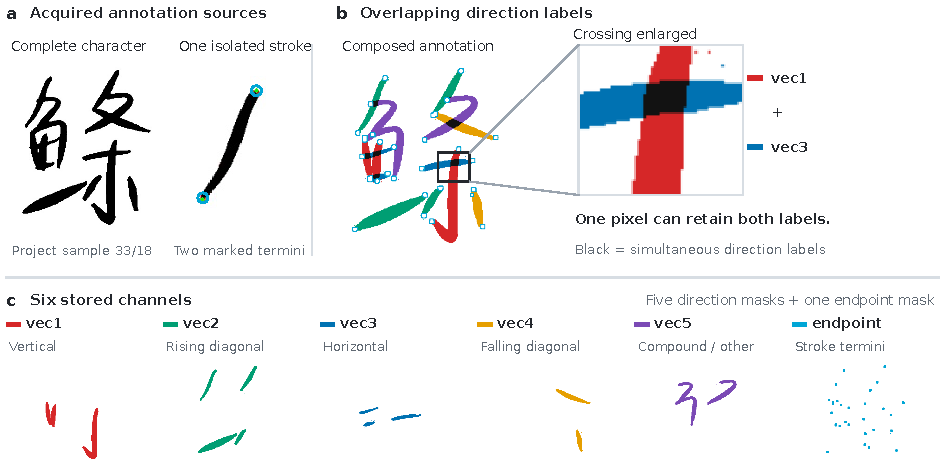
\includegraphics[width=\textwidth]{figures/revision/figure2_channel_definition.pdf}
  \caption{Six-channel overlapping annotation contract on one project
  sample (33/18). (a)~The complete character and one independently acquired
  stroke with two manually marked termini; cyan circles are display outlines.
  (b)~The composed annotation and an enlarged crossing of \(\mathrm{vec1}\)
  and \(\mathrm{vec3}\). Black pixels retain both direction labels rather
  than an exclusive class. (c)~The five direction channels and the endpoint
  channel, shown on a shared crop. The \(\mathrm{vec5}\) family includes
  compound, curved, and other non-cardinal strokes; the endpoint channel is
  the union of manually marked stroke termini, with dilation for display only.
  The software schema stores the channels as
  \((\mathrm{vec1},\ldots,\mathrm{vec5},\mathtt{keypoint})\); the last
  identifier is retained for backward compatibility and denotes this endpoint
  channel.}
  \label{fig:channel-definition}
\end{figure*}

The archive records preserve neither a trustworthy mapping from samples to
writers nor a standardized measure of contributor expertise, so the paper
makes no professional-calligrapher, different-writer, or writer-disjoint
claim.

\subsection{Quality control and split protocols}
\label{sec:data-qc}

Recovery of the acquisition archive yielded 894 sample directories across 43
character identities. Complete six-channel ground truth is available for 840
samples from identities 0--39; the 54 samples of identities 40--42 lack the
character-specific direction mapping and are excluded rather than
pseudo-labelled. A frozen semantic quality-control pass then identified 12
source-image/ground-truth mismatches and 59 non-canonical members of exact
image-and-mask duplicate groups. The two exclusion sets do not overlap,
leaving 769 unique QC-clean observations of 40 identities
(Fig.~\ref{fig:data-resources}a,b). All exclusion decisions were fixed before
the formal model comparison.

\begin{figure*}[!t]
  \centering
  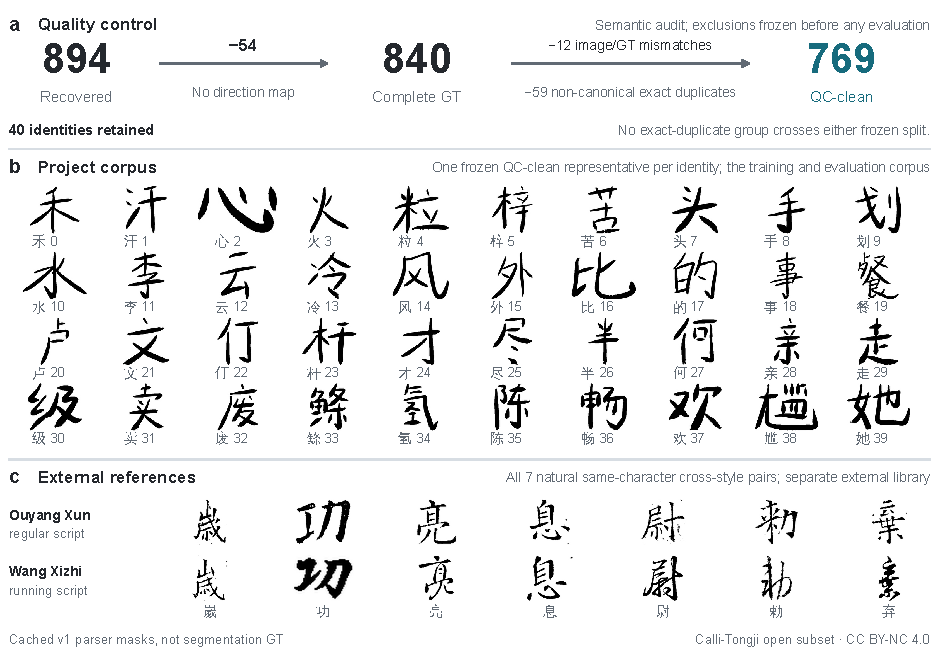
\includegraphics[width=\textwidth]{figures/revision/figure3_dataset_overview.pdf}
  \caption{Data resources and quality control. (a)~Recovery and exclusion
  audit: 54 of 894 recovered samples lack a direction mapping, leaving
  840 with complete six-channel ground truth. Removing 12 image/GT mismatches
  and 59 non-canonical exact duplicates yields 769 QC-clean observations of
  40 identities. No exact-duplicate group crosses either frozen split.
  (b)~One deterministic QC-clean observation per identity (IDs 0--39).
  (c)~All seven natural same-character cross-style pairs in the external
  library, represented by cached v1 parser masks, not segmentation ground
  truth. Source images: Calli-Tongji open subset \cite{yunmo_jixin_2025},
  CC~BY-NC~4.0.}
  \label{fig:data-resources}
\end{figure*}

Figure~\ref{fig:data-resources} shows the same audit graphically:
panel~(a) gives the exclusion flow and the retained identity count,
panel~(b) one deterministic QC-clean observation per retained identity so
that the character coverage of the corpus is visible at a glance, and
panel~(c) the seven natural cross-style pairs of the separate reference
library, whose cached masks are parser outputs rather than annotated ground
truth.

Two split protocols are used. The \emph{standard} assignment was frozen
before quality control by per-character sample index, with the same index
ranges in every identity, and contains 600/120/120 train/validation/test
samples before quality control and 530/119/120 after it; it measures
in-corpus generalization to new instances of seen identities. The
\emph{character-disjoint} assignment was frozen at the identity level before
any formal evaluation, with 28/6/6 disjoint identities and 588/126/126
samples before quality control and 539/114/116 after it; it measures
transfer to identities never seen in training. No exact-duplicate group
crosses either split.

\subsection{External reference library and derived cohorts}
\label{sec:data-references}

The reference-conditioned experiments use 200 approved images from the
publicly downloadable open subset of Calli-Tongji \cite{yunmo_jixin_2025}
(50 calligrapher--script categories with 100 samples each, released under
CC~BY-NC~4.0): the 100 images of the Ouyang Xun regular-script category and
the 100 images of the Wang Xizhi running-script category. Each
reference is parsed once by a frozen SegFormer-B2 checkpoint (version v1,
trained with the recipe of Sect.~\ref{sec:setup-parser} on the
pre-quality-control standard assignment and frozen before the formal
three-seed comparison), and the resulting six binary masks are cached with their provenance. These cached masks are model-derived reference
representations; they are never treated as segmentation ground truth and
never enter parser training.

Two cohorts are derived deterministically from the cached masks. The
\emph{perturbation cohort} applies the nuisance and structural edits of
Sect.~\ref{sec:setup-registration} to every reference, so that registration
and score behaviour can be studied without a second parser inference. The
\emph{cross-reference cohort} contains all seven natural
same-character cross-style pairs that the library supports
(Fig.~\ref{fig:data-resources}c) and 50 different-character negatives selected independently of any model score; the
library contains no same-style, different-instance reference pair. The perturbation cohort also serves as the diagnostic cohort of
Sect.~\ref{sec:setup-diagnostic}, where each known intervention is the
ground truth.

\subsection{Human-rating development cohort}
\label{sec:data-human}

Before any rating was collected, 150 natural same-character,
different-instance pairs were selected from the 769 QC-clean project samples,
three or four per identity, excluding mismatches, exact and suspected near
duplicates, and repeated instances. Pair roles, asset hashes, blinded
identifiers, and display order were frozen, and all automated scores and
source identifiers were hidden from the raters.

Three adult raters independently judged structural similarity on
a five-point ordinal scale, each rating the 150 canonical pairs plus 15
interspersed hidden repeats. The panel comprised two author-raters
with prior calligraphy study, one of whom holds a Level-9 calligraphy
certificate, and one non-author rater with master's-level training in Fine
Arts (Calligraphy). The panel is small, domain-qualified, and partly
author-involved; it is not an independent expert cohort. The main score
comparisons use the annotated masks of both instances, and the paired
direct-ink control uses thresholded source rasters. Neither includes parser
inference, so these comparisons assess score validity without parser error.
The ratings are the ASDS development data of
Sect.~\ref{sec:setup-human}, not an external test set.
